\chapter{Extended Neyman Pearson Test}

\newcommand{\bom}{\boldsymbol{\omega}}
This chapter starts by introducing the Extended Neyman Pearson Framework. Some properties concerning the ENP test are considered, as well as its limitation. Then, the Modified Extended Neyman Pearson (MENP) framework is presented aiming to achieve the largest probability of detection under any possible probability of false alarm constraints. Finally an algorithm for calculating the MENP parameters is considered, and  computer simulation results, which illustrate the performance of the algorithm, are presented. 

%========================Extended Neyman Pearson 
\typeout{}
% chapter 2 section 1
\section{The Extended Neyman Pearson Hypotheses Test}
The theories of hypotheses testing have been a subject of continuous studies over years, and have found applications in various fields such as radar systems, spectrum sensing for cognitive communication systems, and in  medical science \cite{ma2008soft, srinivasan1986distributed, spielman1973refutation}. One type of hypotheses testing problem can be abstracted as  follows: assume $M+1$  hypotheses $H_0$, $H_1$, ..., $H_{M}$, inducing $M+1$  Probability Density Functions (PDFs) on the observable $Y$,
\begin{equation}
\label{equ:hypothesis}
\begin{split}
H_0:\;\;\;\;\;\;\;\;\;&Y \sim f_0(y) \\
H_1:\;\;\;\;\;\;\;\;\;&Y \sim f_1(y)\\
&......\\
H_M:\;\;\;\;\;\;\;\;\;&Y \sim f_M(y)\\
\end{split}
\end{equation}

Based on $y$, a realization of $Y$, the detector needs to decide whether or not it comes from $f_0(y)$. A framework for solving this problem for $M=1$ was introduced in \cite{neyman1933problem} and it is commonly known as Neyman Pearson (NP) testing \cite{neyman1933problem}. The theory of NP testing was further developed for $M \geq 2$ in \cite{wald1939contributions} and \cite{dantzig1951fundamental}.  A comprehensive exposition of such generalized NP testing can be found in \cite{LehmannTest}.

\noindent  \textbf{The Extended Neyman Pearson (ENP) Lemma:}

\textit{
  Let $f_0(x), f_1(x), ..., f_{M}(x)$ be real Borel measurable functions  defined on a finite dimensional Euclidean Space $\mathcal{R}$, such that $\int \limits_\mathcal{R} | f_i(x)|\mathrm{d}x < \infty (i=0, 1,...,M)$.  Suppose that for given constants $c_1,...,c_M$ there exists a class of subsets $\mathcal{S}$, denoted $\mathcal{C}_\mathcal{S}$, such that for every $\mathcal{S} \in \mathcal{C}_\mathcal{S}$ we have
\begin{equation}
\label{one}
\int\limits_\mathcal{S} f_i(x)\mathrm{d}x = c_i, \;\;\;\;\;\;i=1,...,M
\end{equation}
Then:
%No. 1
\\\textnormal{(\rmnum{1})} Among all members of $\mathcal{C}_\mathcal{S}$ there exists one that maximizes
\[
\int \limits_\mathcal{S} f_{0}(x)\mathrm{d}x.
\]
%No.2
\\\textnormal{(\rmnum{2})} A sufficient condition for a member of $\mathcal{C}_\mathcal{S}$ to maximize
\[
\int \limits_\mathcal{S} f_{0}(x)\mathrm{d}x.
\]
is the existence of constants $k_1,...,k_M$ such that
\begin{equation}
\label{2}
f_{0}(x)>\sum\limits_{j=1}^M k_j f_j(x)\;\;\;\;\text{when $x \in \mathcal{S}$}
\end{equation}
\begin{equation}
\label{3}
f_{0}(x)<\sum\limits_{j=1}^M k_j f_j(x)\;\;\;\;\text{when $x \notin \mathcal{S}$}
\end{equation}
%No. 3
\\\textnormal{(\rmnum{3})} If a member of $\mathcal{C}_\mathcal{S}$ satisfies  \textnormal{(\ref{2})} and \textnormal{(\ref{3})} with $k_1,...,k_M\geq0$, then it maximizes
\begin{equation}
\label{4}
\int \limits_\mathcal{S} f_{0}(x)\mathrm{d}x
\end{equation}
among all $\mathcal{S}$ satisfying
\begin{equation}
\label{5}
\int \limits_\mathcal{S} f_i(x)\mathrm{d}x\leq c_i,\;\;\;\;i=1,...,M.
\end{equation}
%no. 4
\\\textnormal{(\rmnum{4})} The set $\mathcal{V}_\mathcal{M}$ of points in $M$-dimensional space whose coordinates are 
\begin{equation}
(\int_{\mathcal{S}}f_1(x)\mathrm{d}x, ..., \int_{\mathcal{S}}f_M(x)\mathrm{d}x)
\end{equation}
for any $\mathcal{S}$ is convex and closed. If $(c_1, ..., c_M)$ is an inner point of $\mathcal{V}_\mathcal{M}$, then a  necessary condition for a member of $\mathcal{C}_\mathcal{S}$ to maximize 
\[
\int \limits_\mathcal{S} f_{0}(x)\mathrm{d}x.
\]
is that there exists $M$ constants $k_1, ..., k_M$ such that \eqref{2} \eqref{3} holds a.e..
}

The associated probability of detection, $P_d$ and false alarms $P_{f_i}$ for a certain subset $\mathcal{S}$ are defined as
\cite{neyman1933problem}, 
\begin{equation}
\begin{split}
P_d &= P(H_0 | H_0) = \int_{\mathcal{S}}f_0(x)\mathrm{d}x\\
P_{f_1} &= P(H_0 | H_1) = \int_{\mathcal{S}}f_1(x)\mathrm{d}x\\
&......\\
P_{f_M} &= P(H_0 | H_M) = \int_{\mathcal{S}}f_M(x)\mathrm{d}x
\end{split}
\end{equation}

 Define the step function
\begin{equation}
   \label{equ: step function}
   u(x) = \begin{cases}
     0\;\;\;\;\;\;&x < 0\\
     0.5\;\;\;\;\;\;&x=0\\
     1\;\;\;\;\;\;&x>0\,,
   \end{cases}
\end{equation}
then for a subset $\mathcal{S}$ satisfying \eqref{2} and \eqref{3} we have:
\begin{equation}
\label{equ: pf and pd}
\begin{split}
&P_d = \int_{-\infty}^{\infty} u(f_0(x) - \sum_{j=1}^{M}k_jf_j(x)) f_0(x)\mathrm{d}x	\,, \\
&P_{f_i} = \int_{-\infty}^{\infty} u(f_0(x) - \sum_{j=1}^{M}k_jf_j(x)) f_i(x) \mathrm{d}x\;\;	 i=1, 2, ..., M\,.
\end{split}
\end{equation}
The relationship between $P_d$ and $P_{f_i}$ can be represented by Receiver Operating Characteristic (ROC) surface \cite{LehmannTest}.

From to \eqref{2} \eqref{3}, the ENP Decision rule $\delta$ is

\begin{equation}
\label{equ: decision rule}
\delta: f_0(x) \substack{H_0 \\ \geq \\ < \\ \bar{H}_0}  \sum_{j=1}^{M} k_jf_j(x)
\end{equation}

From the  \textbf{ENP Lemma}, $\delta$  achieves the largest $P_d$ under the constraints $P_{f_i} = c_i (i = 1, 2, ..., M)$.
When $M=1$, it achieves the largest $P_d$ under the constraint $P_f \leq c$ \cite{LehmannTest}, which is the well known and commonly used form of the NP test.

% notes from Prof. Leib.
For applications in spectrum sensing, $H_0$ denotes the hypothesis that the channel is free and $H_m \;(m=1, ..., M)$ corresponds to the hypothesis that the channel is occupied by the $m$-th primary signal. Although we have $M$ hypotheses, we intend to determine if the channel is free or not. Hence we need  a binary test of deciding $H_0$ versus $\bar{H}_0$ such that $P_d$ is maximized under the constraints $P_{f_m} \leq c_m$ $m = 1, ..., M$. In context of spectrum sensing, $1-P_{f_m}$ can be interpreted as the protection level of the $m-$th primary signal. The larger is this protection level, the smaller is the probability that when the $m-$th signal is active, the test will not detect it and will declare the channel free. In context of spectrum sensing, the solution of the ENP problem maximizes the probability of detecting a free channel under a constraint on the protection level for each primary signal. The protection levels of primary signals can be different and they are guaranteed.


%========================ENP Properties 
\typeout{}
% This is chapter 2 section 2

\section{Properties of ENP Test}
This section presents an example and three Lemmas to illustrate the properties of the ENP test. 

\subsection{An Example}
Assume three hypotheses given as:
\begin{equation}
  \label{2015jan29a2}
\begin{split}
H_0:\;\;\;\;&X \sim \mathcal{N}(-1, 1)\\
H_1:\;\;\;\;&X \sim \mathcal{N}(0, 1)\\
H_2:\;\;\;\;&X \sim \mathcal{N}(1, 1)
\end{split}
\end{equation}
where $\mathcal{N}(\mu, \epsilon^2)$ denotes a Gaussian PDF with mean $\mu$ and variance $\epsilon^2$. In the following, we compute the ROC surface for problem \eqref{2015jan29a2}.  
From \eqref{equ: pf and pd} we can see the expression of $P_{f_1} $, $P_{f_2}$ and $P_d$ can be written in form of  
\begin{equation}
  \begin{split}
	P_{f_1} &= \int_{-\infty}^{\infty}u(f_0(x) - k_1f_1(x) -k_2f_2(x))f_1(x)\mathrm{d}x\\
	P_{f_2} &= \int_{-\infty}^{\infty}u(f_0(x) - k_1f_1(x) -k_2f_2(x))f_2(x)\mathrm{d}x\\
	P_d     &= \int_{-\infty}^{\infty}u(f_0(x) - k_1f_1(x) -k_2f_2(x))f_0(x)\mathrm{d}x\,.
  \end{split}
  \label{2015jan29a1}
\end{equation}

By increasing $k_1$ and $k_2$ from $-30$ to $30$ with step $0.05$ separately, we can calculate the associated $P_{f_1}, P_{f_2}$ and $P_d$ from \eqref{2015jan29a1}. The ROC surface is presented in Fig. \ref{fig: 2.1}. 

\begin{figure}[!t]
\centering
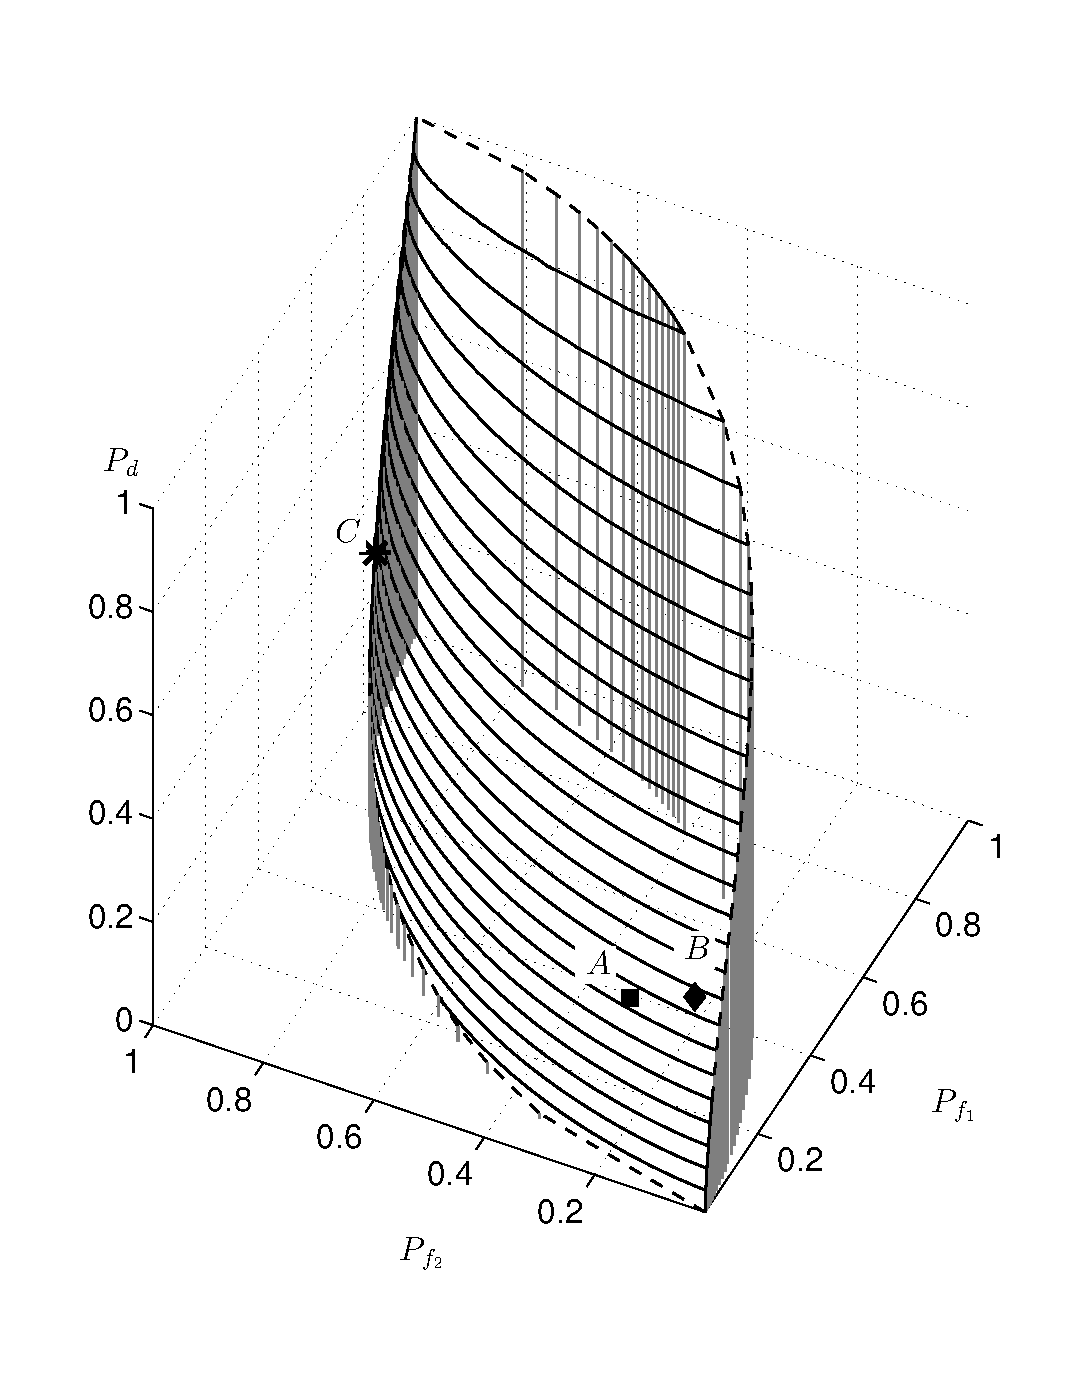
\includegraphics[width = 12cm, height=16cm]{2/c21.eps}
\caption{The ROC surface for $k_1$, $k_2$ range from $-30$ to $30$ with step $0.05$}
\label{fig: 2.1}
\end{figure}

It is interesting to observe that under ENP test framework, for a given $(P_{f_1}, P_{f_2})$  ($P_{f_1}, P_{f_2}\in [0, 1]$) the associated $P_d$ may not exists. This is because for a given $c_1, c_2 \in [0, 1]$, it is possible that there is no decision rule can satisfy
\[
  P_{f_1} = \int_{\mathcal{S}}f_1(x)\mathrm{d}x =  c_1
\]
and
\[
  P_{f_2} = \int_{\mathcal{S}}f_2(x)\mathrm{d}x = c_2
\]
at the same time. In such case, the corresponding $P_d$ does not exist. 
For example, assume $c_1 = 1$ and $c_2 = 0$. In order to satisfy 
\[
  P_{f_1} = \int_{\mathcal{S}}f_1(x)\mathrm{d}x = 1\,,
\]
set $\mathcal{S}$  must  be the whole real line, i.e. $\mathcal{S} = (-\infty, \infty)$. However in such case, we have
\[
  P_{f_2} = \int_{\mathcal{S}}f_2(x)\mathrm{d}x = 1 \neq 0
\]
Hence we can see there is no decision rule can satisfy $P_{f_1} = 1$ and $P_{f_2} = 0$ at the same time, which makes the corresponding $P_d$ do not exist.
Recall in the case of binary hypotheses testing (Traditional Neyman Pearson Test), for a given $P_f \in [0, 1]$, there always exists a corresponding $P_d$. 
% Need to change the coordinates of point A B and C.
% This is because we changed all the figures in 
Now let us consider points $A$ and $B$ on the ROC surface, which are marked with '$\blacksquare$' and '$\blacklozenge$', respectively.  The coordinate of point $A$ is $(P_{f_1}, P_{f_2}, P_d) = (0.0841, 0.1761, 0.2868)$; and the coordinate of point $B$ is  $(P_{f_1}, P_{f_2}, P_d) = (0.0807, 0.0570, 0.3344)$. We can see even through $P_{f_1}$ and $P_{f_2}$ of point $A$ is larger than that of point $B$, the probability of detection of point $A$ is  smaller than that of point $B$.  
Unlike NP test, where $P_d$ is always non-decreasing with $P_f$, in the case of multiple hypotheses testing (Extended Neyman Pearson Test), $P_d$ is not always a non-decreasing function of  $P_{f_i}$ ($i=1, ..., M$).

Finally we consider point $C$ on the ROC surface, which is marked by '$\ast$'. The coordinate of point $C$ is $(P_{f_1}, P_{f_2}, P_d) = (0.7291, 0.9454, 0.3819)$. We can observe, in this case the value of $P_d$ is smaller than the value of $P_{f_1}$ and $P_{f_2}$, i.e. under ENP test framework, $P_d \geq P_{f_i}$  ($i = 1, ..., M$) does not always hold (Qian Zhang arrives at the same conclusion in  \cite{zhang1999design, zhang2000efficient} using a different method). 

\subsection{Three Lemmas for the ENP Test}

Next we presents three lemmas concerning the properties of the ENP test.

\noindent \textbf{Lemma 1}
\noindent \textit{
Let $f_0$, $f_1$, ..., $f_M$ be PDFs defined on set $\mathcal{D}$ and $f_0(x) \neq 0$ holds a.e. on $\mathcal{D}$. For given constants $c_1, ..., c_M \in (0, 1)$, let $\mathcal{C}_\delta$ denote a set of decision rules,  such that for $\delta \in \mathcal{C}_\delta$, we have $P_{f_i} \leq c_i$.
%No. 1
%\\\textnormal{(\rmnum{1})} Among all members of $\mathcal{C}_\mathcal{S}$ there exists one that maximizes $P_d$.
%No.2
If  $\delta^{\ast}$ is a member of $\mathcal{C}_\delta$ and it maximize $P_d$ among all members of $\mathcal{C}_\delta$, then there exists non-negative constants $k_1, ..., k_M$ such that $\delta^\ast$ can be written in form of  
\begin{equation}
f_0(x) \substack{H_0 \\ \geq \\ < \\ \bar{H}_0} \sum_{j=1}^{M}k_jf_j(x)
\end{equation}
Moreover, under decision rule $\delta^\ast$ if  $P_{f_i} < c_i$, then $k_i = 0$. 
}

Qian Zhang also arrives at the conclusion that if $P_{f_i} < c_i$, then $k_i = 0$ in \cite{zhang1999design, zhang2000efficient} through analysing the performance of $P_d$ with respect to $k_i$. In the following we will prove \textbf{Lemma 1} using a mathematical method such that used in \cite{LehmannTest, dantzig1951fundamental} to prove the ENP Lemma (\rmnum{4}).

\noindent\textbf{PROOF}
\newcommand{\bmu}{\boldsymbol{\mu}}
We start by defining 
 some notations for easy presentation.
Define $\mathbf{c}^T = [c_1, c_2, ..., c_M]$, $\boldsymbol{\mu}_0^T = [\mu_1, ..., \mu_M]$, $\mathbf{k}^T = [k_1, k_2, ..., k_M]$ and  $\mathbf{P}_f^T = [P_{f_1}, P_{f_2}, ..., P_{f_M}]$ that are vectors in an $M$ dimensional Euclidean  space. Let $\bmu^T = [\bmu_0, \mu_{M+1}]$ denote a vector in $M+1$ dimensional Euclidean space. 

Let $F(\boldsymbol{\mu}_0)$ denote the largest $P_d$ under the constraints $P_{f_i} = \mu_i\;\;i = 1, ..., M$.
Let $G(\boldsymbol{\mu}_0)$ denote the largest $P_d$ under the constraints $P_{f_i} \leq \mu_i\;\;i = 1, ..., M$.
Let $P_d(\delta)$, $P_{f_i}(\delta)$ denote the $P_d$ and $P_{f_i}$ achieved by using decision rule $\delta$.
By $\mathbf{A} \leq \mathbf{B}$, $\mathbf{A} = \mathbf{B}$ and  $\mathbf{A} \geq \mathbf{B}$ we mean that every element of $\mathbf{A}$ is no larger than, equal to and no smaller than its corresponding element of $\mathbf{B}$, respectively. 
By $\mathbf{A} \neq 0$, we mean that every element of $\mathbf{A}$ is not equal to $0$. 
Let $G'$ denote the hyper surface in $M+1$ dimensional Euclidean Space defined by 
\begin{equation}
 \label{def: G'}
 G' = \{(\bmu_0, \mu_{M+1})  | \bmu_0 \in [0, 1]^M, \mu_{M+1}= G(\bmu_0) \}\,.
\end{equation}
Let $G_s$ denote the set of points in $M+1$ Euclidean space defined as 
\begin{equation}
  \label{2015feb16n1}
G_s =  \{(\boldsymbol{\mu}_0, \mu_{M+1}) | \boldsymbol{\mu}_0\in [0, 1]^M, \mu_{M+1} \in [0, G(\mathbf{\bmu_0})]
    \}\,.
  \end{equation}
  From \eqref{def: G'} and \eqref{2015feb16n1}, it can be seen $G' \in G_s$. Fig. \ref{fig: feb18} depicts the relationship between $G'$ and $G_s$ when $M=2$. In Fig. \ref{fig: feb18}, $G'$ is the surface enclosed by curve $\stackrel\frown{AC}$, curve $\stackrel\frown{AD}$, segment $\overline{OC}$ and segment $\overline{OD}$. Set $G_s$ is the space enclosed by plane $ABC$, plane $ABD$, plane $COD$ and surface $G'$.  

\begin{figure}[!t]
\centering
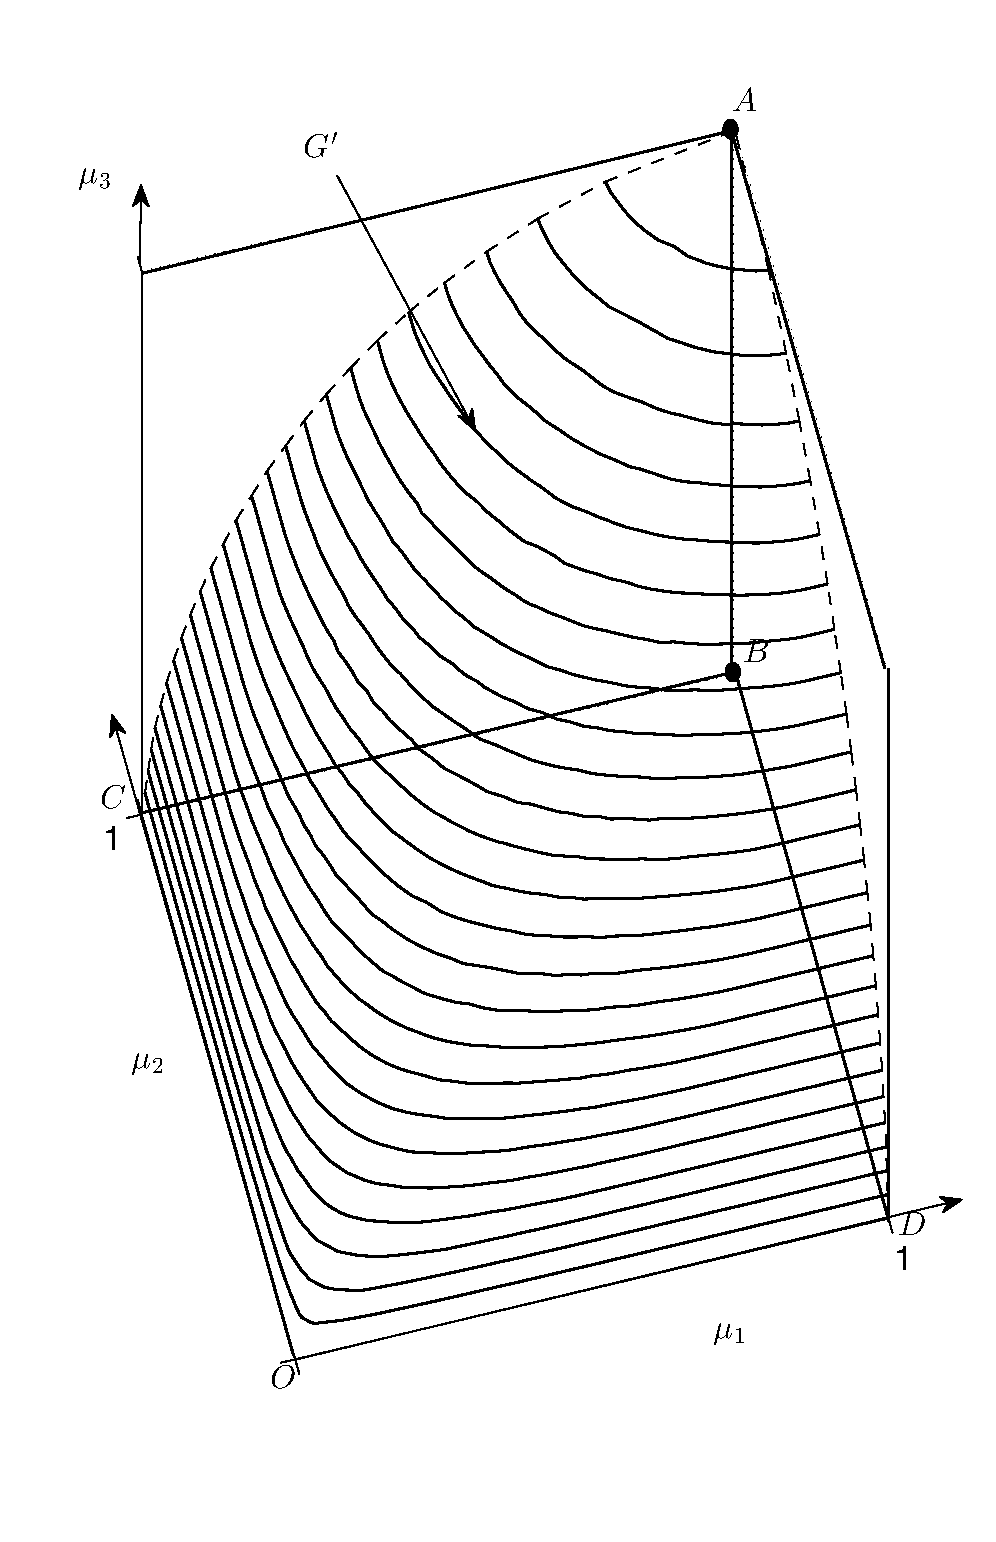
\includegraphics[width = 12cm, height=16cm]{2/example_pic.eps}
\caption{Relationship between $G'$ and $G_s$}
\label{fig: feb18}
\end{figure}
Let us define the set of points in $M+1$ dimensional Euclidean
\begin{equation}
\begin{split}
  \mathcal{N} = \{(\mu_1, \mu_2, ..., \mu_{M+1}) &| \mu_i = \int_{\mathcal{S}}f_i(x)\mathrm{d}x \;\;i=1, ..., M,\\
                                            &  \mu_{M+1}=\int_{\mathcal{S}}f_{0}(x)\mathrm{d}x \;\;\text{ for an $\mathcal{S}$}\}
\end{split}
\end{equation}
We can see that $\mathcal{N}$ is the set of point $(\bmu_0, \mu_{M+1})=(\mathbf{P}_f(\delta), P_d(\delta))$, where $\delta$ is a decision rule. Moreover, from the definition of $\mathcal{N}$ and $F(\bmu_0)$ we can conclude that for a point $(\bmu_0, \mu_{M+1}) \in \mathcal{N}$, we have $\mu_{M+1} \leq F(\bmu_0)$. 
To see it, assume $\mu_{M+1} > F(\bmu_0)$. Then there is a decision rule $\delta$ such that $P_{f_i}(\delta) = \mu_i$ ($i=1, ..., M$) and $P_d(\delta) > F(\bmu_0)$. This is contradictory with the definition of $F(\bmu_0)$. 

The whole proof consists of the following parts: first we prove $G(\boldsymbol{\mu}_0)$ is a convex, non-decreasing function, and when $\boldsymbol{\mu}_0 > 0$, $G(\boldsymbol{\mu}_0) > 0$;
secondly it will be shown that $G_s$ is a convex set and $\mathcal{N} \subseteq G_s$; 
after that we will illustrate for a point $(\mu_1^0, \mu_2^0, ..., \mu_{M+1}^0) \in G'$, there exists a non-negative $\mathbf{k}$ such that 
\[
\mu_{M+1} - \sum_{i=1}^{M}k_i\mu_i \leq \mu_{M+1}^0 - \sum_{i=1}^{M}k_i\mu_i^0
\]
holds for point $(\mu_1, \mu_2, ..., \mu_{M+1}) \in G_s$;
in the end, we will show for $\mathbf{c} \in (0, 1)$, there exists non-negative $\mathbf{k}$ such that the optimal decision rule to achieve the largest $P_d$ under constraint $\mathbf{P}_f \leq \mathbf{c}$ can be written in form of 
\[
f_0(x) \substack{H_0 \\ > \\ < \\ \bar{H}_0} \sum_{i=1}^{M}k_if_i(x)\,.
\]

Firstly we will prove $G(\bmu_0)$ is a convex non-decreasing function for $\bmu_0 \in [0, 1]^M$.
 Let $\boldsymbol{\mu}^1$ and  $\boldsymbol{\mu}^2$ be two points on $G'$ with coordinates $(\boldsymbol{\mu}^1_0, \mu_{M+1}^1)$ and $(\boldsymbol{\mu}^2_0, \mu_{M+1}^2)$, i.e. $\mu_{M+1}^1 = G(\boldsymbol{\mu}_0^1)$ and $\mu_{M+1}^2 = G(\boldsymbol{\mu}_0^2)$. Let $\delta_1$ be a decision rule which can achieve the largest $P_d$ under the constraint $\mathbf{P}_f \leq \boldsymbol{\mu}_0^1$ and $\delta_2$ be a decision rule which can achieve the largest $P_d$ under the constraint $\mathbf{P}_{f} \leq \boldsymbol{\mu}_0^2$. Thus we can see 
 \begin{subequations}
\begin{align}
&\mu_{M+1}^1 = P_d(\delta^1) = G(\boldsymbol{\mu}_0^1)\\
&\mu_{M+1}^2 = P_d(\delta^2)=G(\boldsymbol{\mu}_0^1)\\
&\mathbf{P}_f(\delta^1) \leq \boldsymbol{\mu}^1_0\\
&\mathbf{P}_f(\delta^2) \leq \boldsymbol{\mu}^2_0
\end{align}
 \end{subequations}
 
Construct a new randomized test $\delta^3$, where $\delta^1$ and $\delta^2$ are used with equal probability. With decision rule $\delta^3$, we have 
\begin{subequations}
\begin{align}
\label{1120night1}
&P_d(\delta^3) = 0.5P_d(\delta^1)+0.5P_d(\delta^2) = 0.5G(\bmu_0^1) + 0.5G(\bmu_0^2)\\
&\mathbf{P}_{f}(\delta^3) = 0.5\mathbf{P}_f(\delta^1)+0.5\mathbf{P}_f(\delta^2) \leq 0.5\boldsymbol{\mu}^1_0 + 0.5\boldsymbol{\mu}^2_0
\end{align}
\end{subequations}
Let $\delta'$ denote the optimal decision rule for 
 \begin{equation}
 \begin{split}
 \label{1120t}
 \max&\;\;\;\;P_d\\
 \text{s.t.}&\;\;\;\;\mathbf{P}_f \leq 0.5\boldsymbol{\mu}^1_0 + 0.5\boldsymbol{\mu}^2_0
 \end{split}
 \end{equation}
then obviously $P_d(\delta') \geq P_d(\delta^3)$ (otherwise $\delta'$ cannot be the optimal decision rule for \eqref{1120t}).The optimal $P_d$ of \eqref{1120t} can be written as $G(0.5\boldsymbol{\mu}^1_0 + 0.5\boldsymbol{\mu}^2_0)$, hence we have  
\begin{equation}
\label{1120t2}
G(0.5\boldsymbol{\mu}^1_0 + 0.5\boldsymbol{\mu}^2_0) \geq  P_d(\delta^3).
\end{equation}
Substitute \eqref{1120night1} into above equation, we can see
\begin{equation}
\label{1120t3}
G(0.5\boldsymbol{\mu}^1_0 + 0.5\boldsymbol{\mu}^2_0) \geq 0.5 G(\boldsymbol{\mu}^1_0)+ 0.5 G(\boldsymbol{\mu}^2_0)\,.
\end{equation}
Equation \eqref{1120t3} implies $G(\bmu_0)$ is a convex function for $\bmu_0 \in [0, 1]^M$.

According to the definition of $G(\bmu_0)$, when $\mu_i$ increases, the false alarm constraints are relaxed, 
so the value of $G(\bmu_0)$ will either remain the same or increase. 
This suggests $G(\bmu_0)$ is a non-decreasing function of $\bmu_0$. 
This is not contradictory with the conclusion that 
$P_d$ is not always increasing with $P_{f_i}\;\;(i=1, 2, \cdots, M)$  (we arrived at this conclusion in Chapter 2 section 1.1 on page 12).  This is because $\bmu_0$ is not the probability of false alarms but rather the constraints of the probability of false alarm. 

Next we will show when $\boldsymbol{\mu}_0 > 0^M$, the value of $G(\boldsymbol{\mu}_0)$ is strictly larger than zero.
Let $\delta^\ast$ be the optimal decision rule for $\bmu_0$. By optimal  we mean that this decision rule provides the largest $P_d$ under the constraints $\mathbf{P}_f \leq \bmu_0$, i.e. $P_d(\delta^\ast) = G(\bmu_0)$. Consider two decision rule $\delta^1$ and $\delta^2$ defined as 
\begin{equation}
  \label{2015feb09a4}
  \delta^1:\;\; \begin{cases}
    &x \;\;\;\text{belongs to $H_0$ if } x \in \emptyset \\
    &x \;\;\;\text{belongs to $\bar{H}_0$ if } x \in \mathcal{D}
  \end{cases}
\end{equation}
and
\begin{equation}
  \label{2015feb09a5}
  \delta^2:\;\; \begin{cases}
    &x \;\;\;\text{belongs to $H_0$ if } x \in \mathcal{D} \\
    &x \;\;\;\text{belongs to $\bar{H}_0$ if } x \in \emptyset
  \end{cases}
\end{equation}

From \eqref{2015feb09a4} and \eqref{2015feb09a5} we can see the $P_d$ and $P_{f_i}$ under under decision rule $\delta^1$ and $\delta^2$ can be written as
\begin{equation}
  P_d(\delta^1) = \int_{\emptyset}f_0(x)\mathrm{d}x = 0
\end{equation}
\begin{equation}
    P_{f_i}(\delta^1) = \int_{\emptyset}f_i(x)\mathrm{d}x = 0
\end{equation}
\begin{equation}
    P_d(\delta^2) = \int_{\mathcal{D}}f_0(x)\mathrm{d}x = 1
\end{equation}
\begin{equation}
    P_{f_i}(\delta^2) = \int_{\mathcal{D}}f_i(x)\mathrm{d}x = 1
\end{equation}

Let $\mu_{min} = \min(\mu_1, \mu_2, \cdots, \mu_M)$, since $\bmu_0 > 0^M$, it can be seen $\mu_{min} > 0$. Construct a new randomized test $\delta^3$ where $\delta^1$ and $\delta^2$ are used with probability $1 - \mu_{min} $ and $\mu_{min}$. With decision rule $\delta^3$ we have
\begin{equation}
  P_d(\delta^3) = (1 - \mu_{min})P_d(\delta^1) + \mu_{min}P_d(\delta^2) = \mu_{min} > 0
\end{equation}
\begin{equation}
  P_{f_i}(\delta^3) = (1 - \mu_{min})P_{f_i}(\delta^1) + \mu_{min}P_{f_i}(\delta^2) = \mu_{min} \leq \mu_i \;\;\;\;(i = 1, 2, \cdots, M)
\end{equation}

Hence we can see by using $\delta^3$ we have
\[
  \mathbf{P}_f(\delta^3) \leq \bmu_0\,.
\]
Since $\delta^\ast $ is the optimal decision rule for $\bmu_0$, we can conclude $P_d(\delta^\ast) \geq  P_d(\delta^3) = \mu_{min} >  0$. Since $G(\bmu_0) = P_d(\delta^\ast)$, we can conclude $G(\bmu_0) > 0$ when $\bmu_0 > 0 $. 


In the following, we consider the property of $G_s$. First we will prove that $G_s$ is a convex set. 
Let $\boldsymbol{\mu}^1$ and  $\boldsymbol{\mu}^2$ be two points belongs to $G_s$ with coordinates $(\boldsymbol{\mu}^1_0, \mu_{M+1}^1)$ and $(\boldsymbol{\mu}^2_0, \mu_{M+1}^2)$. According to the definition of $G_s$, we have 
\begin{subequations}
\label{1120t4}
\begin{align}
\label{1120night6}
&0^M \leq \bmu_0^1 \leq 1^M\\
\label{1120night7}
&0^M \leq \boldsymbol{\mu}^2_0 \leq 1^M\\
\label{1120night3}
&0 \leq \mu_{M+1}^1 \leq G(\boldsymbol{\mu}_0^1)\\
\label{1120night4}
&0 \leq \mu_{M+1}^2 \leq G(\boldsymbol{\mu}_0^2)
\end{align}
\end{subequations}

Let $\boldsymbol{\mu}^3$ be the middle point between $\boldsymbol{\mu}^1$ and $\boldsymbol{\mu}^2$ with coordinate $(\bmu_0^3, \mu_{M+1}^3)$, where  
\begin{subequations}
\label{1120t5}
\begin{align}
\label{1120night5}
\bmu_0^3 &= 0.5\boldsymbol{\mu}_0^1 + 0.5 \boldsymbol{\mu}_0^2\\
\label{1120night2}
\mu_{M+1}^3 &= 0.5 \mu_{M+1}^1 + 0.5 \mu_{M+1}^2
\end{align}
\end{subequations}
In the following, we will show $\bmu^3 \in G_s$.  
From \eqref{1120night6}, \eqref{1120night7} and \eqref{1120night5} we can see that
\begin{equation}
\label{equ: 1120n1}
\bmu_0^3 \in [0, 1]^M
\end{equation}
Substituting \eqref{1120night3} \eqref{1120night4} into \eqref{1120night2}, we have
\begin{equation}
  \label{equ:2015feb1a}
0 \leq \mu_{M+1}^3 \leq 0.5 G( \bmu_0^1) + 0.5G(\bmu_0^2)\,.
\end{equation} 
Using \eqref{1120t3} and \eqref{1120night5} with \eqref{equ:2015feb1a} gives,
\begin{equation}
\label{equ: 1120n}
0 \leq \mu_{M+1}^3 \leq G(0.5 \bmu_0^1 + 0.5\bmu_0^2) = G(\bmu_0^3)\,.
\end{equation}
From \eqref{equ: 1120n} and \eqref{equ: 1120n1}, it can be conclude 
 $\bmu^3 \in G_s$, hence $G_s$  is a convex set.  

Next we prove $\mathcal{N} \subseteq G_s$. We need to show that if  $\forall (\mu_1, ..., \mu_{M+1}) \in \mathcal{N}$, then this point also belongs to $G_s$.
Assume $(\mu_1^0, ..., \mu_{M+1}^0)$ is a point in $\mathcal{N}$. 
In previous discussion, it has been shown $\mu_i^0 \in [0, 1]$ ($i = 1, ..., M$) and $\mu_{M+1}^0 \in [0, F(\bmu_0^0)]$, where $\bmu_0^0 = [\mu_1^0, ..., \mu_M^0]$. 
According to the definition of $G(\bmu_0)$ and $F(\bmu_0)$, we can conclude $G(\bmu_0^0) \geq F(\bmu_0^0)$. 
This implies $\mu_{M+1}^0 \in [0, G(\bmu_0^0)]$ and we have  
\begin{equation}
\begin{split}
&\mu_i^0 \in [0, 1]\;\;\;\;(i=1, 2, ..., M)\\
&\mu_{M+1}^0 \in [0, G(\bmu_0^0)]
\end{split}
\end{equation}
The above equation suggests point $(\mu_1^0, ..., \mu_{M+1}^0)$ also belongs to set $G_s$.
Hence we proved $\mathcal{N} \subseteq G_s$. 

In the following we will show for point $(\mu_1^0, \mu_2^0, ..., \mu_{M+1}^0)$ that belongs to $G'$ ($\mu_i^0 \in (0, 1), i = 1, 2, ..., M$), there exists a non-negative $\mathbf{k}$ such that  
\[
\mu_{M+1} - \sum_{i=1}^{M}k_i\mu_i \leq \mu_{M+1}^0 - \sum_{i=1}^{M}k_i\mu_i^0
\]
holds for any $(\mu_1, \mu_2, ..., \mu_{M+1}) \in G_s$, 

Assume $(\mu_0^0, \mu_1^0, ..., \mu_{M+1}^0)$ is a point on the $G'$ surface, i.e. $\mu_{M+1}^0 = G(\bmu_0^0)$, where $\bmu_0^0 = [\mu_1^0, ..., \mu_{M}^0]$. 
Also we assume $\mu_1^0, \mu_2^0, ..., \mu_M^0 \in (0, 1)$. 
According to the definition of $G_s$, for any positive $\epsilon$, point $(\mu_0^0, \mu_1^0, ..., \mu_{M+1}^0+\epsilon) \notin G_s$. Thus point $(\mu_1^0, ..., \mu_{M+1}^0)$ is a boundary point of set $G_s$.  
Since $G_s$ is a convex set and $(\mu_0^0, \mu_1^0, ..., \mu_{M+1}^0)$ is a boundary point of $G_s$,  
there exists an $M+1$-dimensional hyperplane $\Pi$ through this point such that $\Pi$ contains only boundary points of $G_s$ and $G_s$ lies entirely on one sides of $\Pi$  \cite{dantzig1951fundamental}. 
There exists $k_i^0$ ($i=1, ..., M+1$) such that the equation defining $\Pi$ can be written as \cite{dantzig1951fundamental}
\begin{equation}
\label{PI}
k_{M+1}^0\mu_{M+1} - \sum_{i=1}^{M}k_i^0\mu_i = k_{M+1}^0\mu_{M+1}^0 - \sum_{i=1}^{M}k_i^0\mu_i^0
\end{equation}

As  we have proved when $\mu^0_i\neq 0$ ($i=1, ..., M$), $\mu_{M+1}^0 = G(\bmu_0^0) $ is strictly larger than zero. Hence there exists a $\mu_{M+1}' = \frac{\mu_{M+1}^0}{2}$ such that $\mu_{M+1}' \in (0, \mu_{M+1}^0)$. From the definition of $G_s$, it is easy to see that point $(\mu^0_1, ..., \mu^0_M, \mu_{M+1}')$ also belongs to set $G_s$. Besides that, since $\mu^0_i \in (0, 1)$ ($i=1, ..., M$) and $\mu_{M+1}' \in (0, \mu_{M+1}^0)$, it can be concluded that point $(\mu_1^0, \mu_2^0, ..., \mu_{M+1}')$ is an inner point of $G_s$.
From previous discussion, we can see point $(\mu^0_1, ..., \mu^0_M, \mu_{M+1}')$ is not contained in hyperplane $\Pi$, i.e.
\[
k_{M+1}^0\mu_{M+1}' - \sum_{i=1}^{M}k_i^0\mu_i^0 \neq k_{M+1}^0\mu_{M+1}^0 - \sum_{i=1}^{M}k_i^0\mu_i^0
\]
\[
\therefore k_{M+1}^0\mu_{M+1}' \neq k_{M+1}^0\mu_{M+1}^0
\]
\[
\therefore k_{M+1}^0 \neq 0
\]
With $k_i = \frac{k_i^0}{k_{M+1}^0}$, the equation defining the hyperplane $\Pi$ can be written as
\begin{equation}
\label{PI2}
\mu_{M+1} - \sum_{i=1}^{M}k_i\mu_i = \mu_{M+1}^0 - \sum_{i=1}^{M}k_i\mu_i^0\,,
\end{equation}
on equivalently 
\begin{equation}
\label{PI2b}
\mu_{M+1} - \sum_{i=1}^{M}k_i\mu_i - (\mu_{M+1}^0 - \sum_{i=1}^{M}k_i\mu_i^0) = 0\,.
\end{equation}

\cite{planeside} shows $\Pi$ divides the space into two parts, on one side of $\Pi$, points satisfy
\[
\mu_{M+1} - \sum_{i=1}^{M}k_i\mu_i - (\mu_{M+1}^0 - \sum_{i=1}^{M}k_i\mu_i^0) > 0\,;
\]
on the other side of $\Pi$, points satisfy
\[
\mu_{M+1} - \sum_{i=1}^{M}k_i\mu_i - (\mu_{M+1}^0 - \sum_{i=1}^{M}k_i\mu_i^0) < 0\,.
\]

When $(\mu_1, ... ,\mu_M, \mu_{M+1})=(\mu_1^0, ..., \mu_M^0, 0)$, the left-hand of \eqref{PI2} is smaller than the right-hand, i.e.
\begin{equation}
  \begin{split}
 \mu_{M+1} - \sum_{i=1}^{M}k_i\mu_i < \mu_{M+1}^0 - \sum_{i=1}^{M}k_i\mu_i^0\\
 \mu_{M+1} - \sum_{i=1}^{M}k_i\mu_i - (\mu_{M+1}^0 - \sum_{i=1}^{M}k_i\mu_i^0) < 0\,.
 \end{split}
  \label{2015feb02a1}
\end{equation}
 Since $\mu_i^0 \in (0, 1)$, from the definition of $G_s$, we can see that point $(\mu_1, ... ,\mu_M, \mu_{M+1})=(\mu_1^0, ..., \mu_M^0, 0)$ belongs to $G_s$. 
Since point $(\mu_1, ... ,\mu_M, \mu_{M+1})=(\mu_1^0, ..., \mu_M^0, 0)$ satisfies \eqref{2015feb02a1} and since $G_s$ lies entirely on one side of hyper plane $\Pi$, to make all points belonging to $G_s$ lies on the same side of $\Pi$ as point $(\mu_1, ... ,\mu_M, \mu_{M+1})=(\mu_1^0, ..., \mu_M^0, 0)$ does, we must have
%Since $G_s$ lies entirely on one side of \eqref{PI2}, and since when $(\mu_1, ... ,\mu_M, \mu_{M+1})=(\mu_1^0, ..., \mu_M^0, 0)$, the left-hand of \eqref{PI2} is smaller than the right-hand, we must have 
\begin{equation}
\mu_{M+1} - \sum_{i=1}^{M}k_i\mu_i -  ( \mu_{M+1}^0 - \sum_{i=1}^{M}k_i\mu_i^0) \leq 0
\label{PI3}
\end{equation}
on equivalently,
\[
\mu_{M+1} - \sum_{i=1}^{M}k_i\mu_i \leq   \mu_{M+1}^0 - \sum_{i=1}^{M}k_i\mu_i^0
\]
for all the points belong to $G_s$ \cite{dantzig1951fundamental, planeside}. 

Up to now, we have proved that if  $(\bmu_0^0, \mu_{M+1}^0) \in G'$ and $\bmu_0^0 \in (0, 1)^M$, there exists constants $k_1$, ..., $k_M$ such that
\begin{equation}
\mu_{M+1} - \sum_{i=1}^{M}k_i\mu_i \leq \mu_{M+1}^0 - \sum_{i=1}^{M}k_i\mu_i^0
\label{PPI3}
\end{equation}
holds for  $(\mu_1, \mu_2, ...\mu_{M+1}) \in G_s$. In the following, we will show that the constants $k_i$ in \eqref{PPI3} must be non-negative.   

Now consider another point on $G'$ with coordinate $(\mu_1^0, ..., \mu_l^0+\epsilon, ..., \mu_M^0, \mu_{M+1}')$, where $\epsilon > 0$ and $l$ is an integer between $1$ and $M$.  Since both points $(\mu_1^0, ..., \mu_l^0, ..., \mu_M^0, \mu_{M+1}^0)$ and $(\mu_1^0, ..., \mu_l^0+\epsilon, ..., \mu_M^0, \mu_{M+1}')$ lies on $G'$, we can conclude $G([\mu_1^0, ..., \mu_l^0, ...., \mu_M^0]) = \mu_{M+1}^0$ and $G([\mu_1^0, ..., \mu_l^0 + \epsilon, ...., \mu_M^0]) = \mu_{M+1}'$. As we proved $G(\bmu_0)$ is a non-decreasing function, we must have  $\mu_{M+1}' \geq \mu_{M+1}^0$.

Substituting $(\mu_1^0, ..., \mu_l^0+\epsilon, ..., \mu_M^0, \mu_{M+1}')$ into the left side of \eqref{PPI3}, we have
\begin{equation}
\mu_{M+1}' - k_1\mu_1^0 - ... - k_l(\mu_l^0+\epsilon)- ... - k_M\mu_M^0 \leq \mu_{M+1}^0 - k_1\mu_1^0 - ... - k_l\mu_l^0- ... - k_M\mu_M^0
\end{equation}
\begin{equation}
\therefore \mu_{M+1}' - k_l(\mu_l^0+\epsilon)\leq \mu_{M+1}^0 - k_l\mu_l^0
\end{equation}
\begin{equation}
\mu_{M+1}' - \mu_{M+1}^0 \leq k_l\epsilon
\end{equation}
\begin{equation}
\therefore k_l \geq \frac{\mu_{M+1}' - \mu_{M+1}^0}{\epsilon} \geq 0 \;\;\;\;l = 1, 2, \cdots, M
\label{2015feb16a1}
\end{equation}
From \eqref{2015feb16a1} we can see that the constants $k_l$ ($l = 1, 2, \cdots, M$) in \eqref{PPI3} are non-negative.
As we have proved if  $(\bmu_0^0, \mu_{M+1}^0) \in G'$ and $\bmu_0^0 \in (0, 1)^M$, there exists constants $k_1, ..., k_M$ such that  
\begin{equation}
\mu_{M+1} - \sum_{i=1}^{M}k_i\mu_i \leq \mu_{M+1}^0 - \sum_{i=1}^{M}k_i\mu_i^0
\label{PPI32015bc}
\end{equation}
holds for  $(\mu_1, \mu_2, ...\mu_{M+1}) \in G_s$ and the constants $k_1, k_2, \cdots, k_M$ are non-negative,  
we can conclude 
if  $(\bmu_0^0, \mu_{M+1}^0) \in G'$ and $\bmu_0^0 \in (0, 1)^M$, there exists constants $k_1, ..., k_M \geq 0 $ such that  
\begin{equation}
\mu_{M+1} - \sum_{i=1}^{M}k_i\mu_i \leq \mu_{M+1}^0 - \sum_{i=1}^{M}k_i\mu_i^0
\label{PPI32015b}
\end{equation}
holds for  $(\mu_1, \mu_2, ...\mu_{M+1}) \in G_s$. 

For the given constants $\mathbf{c}$ ($\mathbf{c} \in (0, 1)^M$), 
 assume a decision rule $\delta^\ast$  achieves the largest $P_d$  while keeping $\mathbf{P}_f \leq \mathbf{c}$. In the following we will prove there exists non-negative $\mathbf{k}$  such that $\delta^\ast$ can be written in form of 
\[
f_0(x) \substack{H_0 \\ > \\ < \\ \bar{H}_0 } \sum_{i=1}^{M}k_if_i(x)\,.
\]

Let $\bmu_0 = \mathbf{c}$, according to the definition of $G'$, we can see $(\mathbf{c},G(\mathbf{c})) \in G'$.  As $\delta^\ast $ achieves the largest $P_d$ under constraint $\mathbf{P}_f \leq \mathbf{c}$, from the definition of $G(\bmu_0)$ we can see $P_{d}(\delta^\ast) = G(\mathbf{c})$. 

Since we have proved if $(\bmu_0^0, \mu_{M+1}^0) \in G'$ and $\bmu_0^0 \in (0, 1)^M$, there exists non-negative constants $k_1$, ..., $k_M$ such that
\begin{equation}
\mu_{M+1} - \sum_{i=1}^{M}k_i\mu_i \leq \mu_{M+1}^0 - \sum_{i=1}^{M}k_i\mu_i^0
\label{PPI32015}
\end{equation}
holds for all points belonging $G_s$ and $(\mathbf{c},G(\mathbf{c})) \in G'$, we can see there exists non-negative $\mathbf{k}$ such that  

%According to the definition of $G(\bmu_0)$, we can see $P_d(\delta^\ast) = G(\mathbf{c})$. Since $(\mathbf{c}, G(\mathbf{c}))$is a point on the hyper surface $G'$,  there exists non-negative $\mathbf{k}$ such that 
\begin{equation}
\label{TEMP}
\mu_{M+1} - \sum_{i=1}^{M}k_i\mu_i \leq G(\mathbf{c}) - \sum_{i=1}^{M}k_ic_i
\end{equation}
holds for $(\mu_1, \mu_2, ..., \mu_{M+1}) \in G_s$.
Since $P_{f_i}(\delta^\ast) \leq c_i$ (for $i=1, ..., M$) and $k_i \geq 0$, we know
\[
k_ic_i \geq k_iP_{f_i}(\delta^\ast)
\]
\[
\therefore \sum_{i=1}^{M}k_ic_i \geq \sum_{i=1}^{M}k_iP_{f_i}(\delta^\ast)
\]
Hence we have
\begin{equation}
\label{con: 1}
G(\mathbf{c}) - \sum_{i=1}^{M}k_ic_i \leq G(\mathbf{c}) - \sum_{i=1}^{M}k_iP_{f_i}(\delta^\ast)\,.
\end{equation}
From \eqref{TEMP} and \eqref{con: 1}, we have 
\begin{equation}
\label{equ: TEMP3}
\mu_{M+1} - \sum_{i=1}^{M}k_i\mu_i \leq G(\mathbf{c}) - \sum_{i=1}^{M}k_ic_i \leq G(\mathbf{c}) - \sum_{i=1}^{M}k_iP_{f_i}(\delta^\ast)
\end{equation}
\begin{equation}
\label{ASD}
\therefore \mu_{M+1} - \sum_{i=1}^{M}k_i\mu_i \leq G(\mathbf{c}) - \sum_{i=1}^{M}k_iP_{f_i}(\delta^\ast)
\end{equation}
Substitute $G(\mathbf{c}) = P_d(\delta^\ast)$ into \eqref{ASD}, 
\begin{equation}
\label{TEMP2}
\mu_{M+1} - \sum_{i=1}^{M}k_i\mu_i \leq P_d(\delta^\ast) - \sum_{i=1}^{M}k_iP_{f_i}(\delta^\ast)\,,
\end{equation}
where $(\mu_0, ..., \mu_{M+1}) \in G_s$.

Since $\mathcal{N} \subseteq G_s$, \eqref{TEMP2} also holds for a point belonging to $\mathcal{N}$.
According to the definition of $\mathcal{N}$, for $(\mu_1, \mu_2, ..., \mu_{M+1} \in \mathcal{N})$, we have  
\begin{equation}
\label{def: mu}
\begin{cases}
\mu_i = \int_{\mathcal{S}}f_i(x)\mathrm{d}x \;\;\;\;i = 1, ..., M\\
\mu_{M+1} = \int_{\mathcal{S}}f_{0}(x)\mathrm{d}x
\end{cases}
\end{equation}
where $\mathcal{S}$ can be any subset of domain $\mathcal{D}$. 

$P_{f_i}(\delta^\ast)$ and $P_{d}(\delta^\ast)$ can be written as
\begin{equation}
\label{def: pfd}
\begin{cases}
P_{f_i}(\delta^\ast) = \int_{\mathcal{S}^\ast}f_i(x)\mathrm{d}x\;\;\;\;i=1, ..., M\\
P_d(\delta^\ast) = \int_{\mathcal{S}^\ast}f_0(x)\mathrm{d}x
\end{cases}
\end{equation}
Substituting \eqref{def: mu} and \eqref{def: pfd} into \eqref{TEMP2}, we have: 
\[
\int_{\mathcal{S}}f_{0}(x)\mathrm{d}x - \sum_{i=1}^{M}k_i\int_{\mathcal{S}}f_i(x)\mathrm{d}x \leq \int_{\mathcal{S}^\ast}f_{0}(x)\mathrm{d}x - \sum_{i=1}^{M}k_i\int_{\mathcal{S}^\ast}f_i(x)\mathrm{d}x
\]
\[
\therefore 
\int_{\mathcal{S}}f_{0}(x)\mathrm{d}x - \sum_{i=1}^{M}\int_{\mathcal{S}}k_if_i(x)\mathrm{d}x \leq \int_{\mathcal{S}^\ast}f_{0}(x)\mathrm{d}x - \sum_{i=1}^{M}\int_{\mathcal{S}^\ast}k_if_i(x)\mathrm{d}x
\]
\begin{equation}
\label{TEMP4}
\therefore \int_{\mathcal{S}}(f_{0}(x)- \sum_{i=1}^{M}k_if_{i}(x))\mathrm{d}x \leq \int_{\mathcal{S}^\ast}(f_{0}(x)- \sum_{i=1}^{M}k_if_{i}(x))\mathrm{d}x 
\end{equation}
The integrand of the left-hand \eqref{TEMP4} and right-hand \eqref{TEMP4} are the same. In order to make \eqref{TEMP4} holds for all set $\mathcal{S}$,  
 $\mathcal{S}^\ast$ must  maximize 
\begin{equation}
\int_{\mathcal{S}}(f_{0}(x)\mathrm{d}x - \sum_{i=1}^{M}k_if_i(x))\mathrm{d}x
  \label{2015feb2a3}
\end{equation}
among all $\mathcal{S}$. To maximize \eqref{2015feb2a3}, $\mathcal{S}^\ast$ should include all the integral set when $f_{0}(x)- \sum_{i=1}^{M}k_if_{i}(x) > 0$ and exclude the integral set when $f_{0}(x)- \sum_{i=1}^{M}k_if_{i}(x) < 0$, i.e.   
 $\mathcal{S}^\ast$ satisfies
\[
x \in \mathcal{S}^\ast\;\;\;\;\text{if}\;\;\;\;f_{0}(x)- \sum_{i=1}^{M}k_if_{i}(x) > 0
\]
\[
x \notin \mathcal{S}^\ast\;\;\;\;\text{if}\;\;\;\;f_{0}(x)- \sum_{i=1}^{M}k_if_{i}(x) < 0
\]

Hence we can conclude that for a given vector of constraints for $\mathbf{P}_f$, denoted as $\mathbf{c} \in (0, 1)^M$, there exists a set of non-negative $\mathbf{k}$ such that 
the optimal decision rule can be written as 
\[
f_0(x) \substack{H_0 \\ > \\ < \\ \bar{H}_0 } \sum_{i=1}^{M}k_if_i(x)\,.
\]

Moreover, since \eqref{TEMP} holds for any point $(\mu_1, \mu_2, ..., \mu_{M+1}) \in \mathcal{N}$ and $(\mathbf{P}_f(\delta^\ast), P_d(\delta^\ast)) \in \mathcal{N}$, we can conclude 
\begin{equation}
P_d(\delta^\ast) - \sum_{i=1}^{M}k_iP_{f_i}(\delta^\ast) \leq G(\mathbf{c}) - \sum_{i=1}^{M}k_ic_i
\end{equation}
As we have shown $G(\mathbf{c}) = P_d(\delta^\ast)$, the above equation can be written as
\begin{equation}
 G(\mathbf{c}) - \sum_{i=1}^{M}k_ic_i \geq G(\mathbf{c}) - \sum_{i=1}^{M}k_iP_{f_i}(\delta^\ast)
\label{TEMP5}
\end{equation}
From \eqref{con: 1} and \eqref{TEMP5}  we can conclude
\[
G(\mathbf{c}) - \sum_{i=1}^{M}k_iP_{f_i}(\delta^\ast) =  G(\mathbf{c}) - \sum_{i=1}^{M}k_ic_i
\]
\[
\therefore  \sum_{i=1}^{M}k_iP_{f_i}(\delta^\ast) =  \sum_{i=1}^{M}k_ic_i
\]
Since $k_iP_{f_i}(\delta^\ast) \leq k_ic_i$ (for $i=1, ..., M$), the above equation can be fulfilled only if $k_iP_{f_i}(\delta^\ast) = k_ic_i$ (for $i=1, ..., M$). When for a certain $i$ $P_{f_i}(\delta^\ast) < c_i$, then $k_i$ must be zero.

Q.E.D.

Upon examination  the optimal decision rule for a given probability of false alarm constraints, in the following we consider properties of the ROC surface, embodied by two lemmas with proof.  

\noindent \textbf{Condition 1}
\textit{
\noindent Let $f_i(x) \;\;i=0, 1, ..., M$ be the PDF induced by hypothesis $H_i$, and define $g(x) = f_0(x) - \sum_{j=1}^{M} k_jf_j(x)$ where $k_i$  ($i = 1, 2, ..., M$) are real numbers. Let $\mathcal{D} \in \mathbb{R}$ be an open set such that $\int_{\bar{\mathcal{D}}}f_i(x)=0\;\;i = 1, 2, ..., M$. Furthermore,  if $x_0$ is a solution  for $g(x) = 0 \;\;(x \in \mathcal{D})$, then there exists an integer $n$ such that  the $n$-th order derivative of $g(x_0)$ is not equal to zero $(g^{(n)}(x_0) \neq 0)$.
}

\noindent \textbf{Lemma 2}
\textit{
\noindent Under}
\textbf{Condition 1}
\textit{, let $\mathbf{P}$ be a point with coordinate $(P_d, P_{f_1}, ..., P_{f_M})$ on the ROC surface of the EPN test. If there exists a tangent hyperplane at $\mathbf{P}$, then its normal is parallel to the vector $\mathbf{n} = (-1, k_1, ..., k_M)$, where $k_i$ are the parameters of the ENP test achieving $\mathbf{P}$.
}

\noindent\textbf{PROOF}
Define $\mathbf{k} = [k_1, k_2, ..., k_M]^T$ and $\mathbf{P}_f = [P_{f_1}, P_{f_2}, ..., P_{f_M}]^T$. Since both $P_d$ and $\mathbf{P}_f$ are functions of $\mathbf{k}$, $\mathbf{P}_f(\mathbf{k}_0)$ denotes the value of $\mathbf{P}_f$ when $\mathbf{k} = \mathbf{k}_0$ and $P_d(\mathbf{k}_0)$ denotes the value of $P_d$ when $\mathbf{k} = \mathbf{k}_0$. Using Taylor's expansion \cite{zill2011advanced} for $\mathbf{P}_f$ and $P_d$,
\begin{equation}
\label{pro: pd}
P_d = P_d(\mathbf{k}_0) + \frac{\mathrm{d}P_d}{\mathrm{d}\mathbf{k}^T}\bigg{|}_{\mathbf{k}=\mathbf{k_0}}(\mathbf{k} - \mathbf{k}_0)
+ o(\mathbf{k} - \mathbf{k}_0)
\end{equation}

\begin{equation}
\label{pro: pf}
\mathbf{P}_f = \mathbf{P}_f(\mathbf{k}_0) + \frac{\mathrm{d}\mathbf{P}_f}{\mathrm{d}\mathbf{k}^T}\bigg{|}_{\mathbf{k}=\mathbf{k_0}}(\mathbf{k} - \mathbf{k}_0)
+ o(\mathbf{k} - \mathbf{k}_0)
\end{equation}
here $\mathbf{k} \rightarrow \mathbf{k}_0$.

Consider the hyperplane $y$ as a function of $\mathbf{x}$ defined by
\begin{equation}
\label{pro: y}
y = P_d(\mathbf{k}_0) + \frac{\mathrm{d}P_d}{\mathrm{d}\mathbf{k}^T}\bigg{|}_{\mathbf{k}=\mathbf{k_0}}(\mathbf{z} - \mathbf{k}_0)
\end{equation}
\begin{equation}
\label{pro: x}
\mathbf{x} = \mathbf{P}_f(\mathbf{k}_0) + \frac{\mathrm{d}\mathbf{P}_f}{\mathrm{d}\mathbf{k}^T}\bigg{|}_{\mathbf{k}=\mathbf{k_0}}(\mathbf{z} - \mathbf{k}_0)
\end{equation}
The above equations construct a tangent hyperplane for the ROC surface at point $(P_d(\mathbf{k}_0), \mathbf{P}_f^T(\mathbf{k}_0))$. Combining both equations  we get

\begin{equation}
\label{pro : y2}
y = P_d(\mathbf{k}_0) + \frac{\mathrm{d}P_d}{\mathrm{d}\mathbf{k}^T}\bigg{|}_{\mathbf{k}=\mathbf{k_0}}(
\frac{\mathrm{d}\mathbf{P}_f}{\mathrm{d}\mathbf{k}^T}\bigg{|}_{\mathbf{k}=\mathbf{k_0}}
)^{-1} (\mathbf{x} - \mathbf{P}_f(\mathbf{k}_0))
\end{equation}
Hence the normal for point $(P_d(\mathbf{k}_0), \mathbf{P}_f^T(\mathbf{k}_0))$ on ROC surface can be written as
\begin{equation}
\label{vec: normal}
[-1, \frac{\mathrm{d}P_d}{\mathrm{d}\mathbf{k}^T}\bigg{|}_{\mathbf{k}=\mathbf{k_0}}(
\frac{\mathrm{d}\mathbf{P}_f}{\mathrm{d}\mathbf{k}^T}\bigg{|}_{\mathbf{k}=\mathbf{k_0}}
)^{-1}
].
\end{equation}

In the following, we will prove $ \frac{\mathrm{d}P_d}{\mathrm{d}\mathbf{k}^T}(
\frac{\mathrm{d}\mathbf{P}_f}{\mathrm{d}\mathbf{k}^T}
)^{-1} = \mathbf{k}^T
$, which can be written as
\begin{equation}
\label{pro: vec}
\frac{\mathrm{d}P_d}{\mathrm{d}\mathbf{k}^T} = \mathbf{k}^T \frac{\mathrm{d}\mathbf{P}_f}{\mathrm{d}\mathbf{k}^T}
\end{equation}
which in component form can be written as 
\begin{equation}
\label{pro: component}
\frac{\partial P_d}{\partial k_i} - \sum_{n=1}^{M}k_n\frac{\partial P_{f_n}}{\partial k_i} = 0 \;\;\;\;(i=1, 2, ..., M).
\end{equation}
Using \eqref{equ: pf and pd} and calculating the  partial derivatives results in
\begin{equation}
\label{pro: Pf par k}
\frac{\partial P_{f_n}}{ \partial k_i} = - \int_{\mathcal{D}}\delta (f_0(x) - \sum_{j=1}^{M}k_jf_j(x))f_i(x)f_n(x) \mathrm{d}x\,,
\end{equation}
\label{pro: Pd par k}
\begin{equation}\frac{\partial P_d}{ \partial k_i} = - \int_{\mathcal{D}}\delta (f_0(x) - \sum_{j=1}^{M}k_jf_j(x))f_i(x)f_0(x) \mathrm{d}x\,,
\end{equation}
where $\delta(\bullet)$ is Dirac's delta function defined as following,

\begin{equation}
\label{pro: delta}
\delta(x) = \substack{\lim \\ \epsilon \rightarrow 0} \begin{cases}
\frac{1}{\epsilon}\;\;\;\;&\text{when} \;\;x \in (-\frac{\epsilon}{2}, \frac{\epsilon}{2})\\
0\;\;\;\;&\text{otherwise}
\end{cases} \;\;\;\;
\end{equation}

Defining $g(x) = f_0(x) - \sum_{j=1}^{M} k_jf_j(x)$, \eqref{pro: component} can be written as $\int_{\mathcal{D}}\delta(g(x))g(x)f_n(x)\mathrm{d}x = 0, n = 1, ..., M$.

When $g(x) \neq 0$, we have $\delta(g(x)) = 0$ and $\delta(g(x))g(x)f_i(x) = 0$.   When  $g(x) = 0$, we can solve the equation according to the definition of $\delta(\bullet)$ and consider
\begin{equation}
\label{pro: important}
\int_{\{x|g(x)\in (-\frac{\epsilon}{2}, \frac{\epsilon}{2})\}} \frac{1}{\epsilon} g(x)f_n(x) \mathrm{d}x\;\;\;\;n= 1, ..., M
\end{equation}

Since when $g(x) \in (-\frac{\epsilon}{2}, \frac{\epsilon}{2})$, $|g(x)| < \frac{\epsilon}{2}$,
\begin{equation}|
\int_{\{x|g(x)\in (-\frac{\epsilon}{2}, \frac{\epsilon}{2})\}} \frac{1}{\epsilon} g(x)f_i(x) \mathrm{d}x | <
\int_{\{x|g(x)\in (-\frac{\epsilon}{2}, \frac{\epsilon}{2})\}} \frac{1}{2}f_i(x) \mathrm{d}x
\end{equation}

When $\epsilon$ is small enough, we have 
\[
  g(x) \in (-\frac{\epsilon}{2}, \frac{\epsilon}{2}) \Leftrightarrow  x \in (x_0 - \frac{\triangle x}{2}, x_0 + \frac{\triangle x}{2})
\]
when $x_0 $ is such that $g(x_0) = 0$, and $\triangle x \rightarrow 0$ when $\epsilon \rightarrow 0$. 

Hence when $\epsilon \rightarrow 0$ we have 

%define
\def \LEFT{ x_s
  -\left(\frac{n!\varepsilon}{2|g^{(n)}(x_s)|}\right)^{\frac{1}{n}}}
  \def \RIGHT{ x_s
  +\left(\frac{n!\varepsilon}{2|g^{(n)}(x_s)|}\right)^{\frac{1}{n}}}
%end define
\begin{equation}
\int_{\{x|g(x)\in (-\frac{\epsilon}{2}, \frac{\epsilon}{2})\}} \frac{1}{2}f_i(x) \mathrm{d}x \rightarrow
f_i(x_0)\bigtriangleup x \rightarrow 0
\end{equation}

Using the above two conclusions for $g(x) = 0$ and $g(x) \neq 0$, we get
\begin{equation}
\int_{\mathcal{D}} \delta (g(x)) g(x)f_i(x) \mathrm{d}x = 0
\end{equation}
proving that \eqref{pro: component} holds.

Q.E.D.

\noindent \textbf{Lemma 3}
\textit{
\noindent
Under}
\textbf{Condition 1}
\textit{, let $\mathbf{P}$ be a point on the ROC surface. Then $\frac{\partial P_d}{\partial P_{f_i}} \bigg|_P = k_i$, where $k_i$ are the parameters of ENP test achieving $\mathbf{P}$.
}

\noindent\textbf{PROOF}
The expression of tangent hyper surface for point $(P_d^0, P_{f_1}^0, ..., P_{f_M}^0)$ on the ROC hyper surface can be written as
\begin{equation}
P_d = P_d^0 + \sum_{i=1}^{M} \frac{\partial P_d}{\partial P_{f_i}}\bigg|_{P_{f_i} = P_{f_i}^0}(P_{f_i} - P_{f_i}^0)\,.
\end{equation}
Hence the normal at this point is

 $\mathbf{n} = [-1, \frac{\partial P_d}{\partial P_{f_1}}, \frac{\partial P_d}{\partial P_{f_2}}, ..., \frac{\partial P_d}{\partial P_{f_M}}]$. Since we have proved that  the normal for this point is $\mathbf{n} = [-1, k_1, k_2, ..., k_M]$, we must have
\begin{equation}
\frac{\partial P_d}{\partial P_{f_i}}\bigg|_{P} = k_i
\end{equation}

Q.E.D.


%========================Relationship between Neyman Pearson and Bayesian 
\typeout{}
\section{Relationship to Bayesian Hypotheses Test}
Upon examination the properties of ENP Test, this section will present the relationship between ENP Test and Bayesian Test. 

Consider the following $M+1$ hypotheses concerning an observation of $X$
\begin{equation}
\label{equ: 2 pdf}
\begin{split}
H_0:\;\;\;\;&X \sim f_0(x)\\
H_1:\;\;\;\;&X \sim f_1(x)\\
&......\\
H_{M}:\;\;\;\;&X \sim f_M(x)\,,
\end{split}
\end{equation}
where $f_i(x)$ ($i=0, 1, ..., M$) are Probability Density Functions (PDFs). 
Let $\pi_0, \pi_1, ..., \pi_M$ be the probability of occurrences of hypotheses $H_0$, $H_1$, ..., $H_M$, respectively. 
Based on $x$, a realization of $X$, a Bayesian Test $\delta_B$ is used to discriminate which hypothesis it comes from.  
Let $C_{ij}$ denote the cost incurred by choosing hypothesis $H_i$ when hypothesis $H_j$ is true. 
Let $\mathcal{C}_i$ ($i=1, ..., M$) denote a subset of $\mathbb{R}$ such that under decision rule $\delta_B$ we choose $H_i$ when $x \in \mathcal{C}_i$. 
Let $P_i(\mathcal{C}_j)$ denote the integration of $f_i(x)$ over subset $\mathcal{C}_j$, i.e. 
\[
P_i(\mathcal{C}_j) = \int_{\mathcal{C}_j} f_i(x)\mathrm{d}x\,.
\]
Before we process, we make following assumption:
\\(1) $C_{ij} = 0$ when $i \neq 0$ and $j \neq 0$
\\(2) $C_{10} = C_{20} = ... = C_{M0}$

In the following, we consider the form of $\delta_B$ under such assumption.
Let $a_0 = C_{10} = C_{20} = ... = C_{M0}$ and $a_i = C_{0i}$ ($i= 1, 2, ..., M$).
The conditional risk for Bayesian Test can be written as 
\begin{subequations}
\label{r0}
\begin{align}
\begin{split}
R_0(\delta_B) &= C_{00}P_0(\mathcal{C}_0) + C_{10}P_0(\mathcal{C}_1) + ... +  C_{M0}P_0(\mathcal{C}_M)\\
&= a_0P_0(\mathcal{C}_1) + a_0P_0(\mathcal{C}_2) + ... + a_0P_0(\mathcal{C}_M)\\
&= a_0P_0(\mathcal{C}_1\cup \mathcal{C}_2 \cup ... \cup \mathcal{C}_M)\\
&= a_0P_0(\bar{\mathcal{C}_0})\\
&= a_0(1 - P_0(\mathcal{C}_0))\\
&= a_0(1 - \int_{\mathcal{C}_0}f_0(x)\mathrm{d}x)\\
\end{split}
\begin{split}
R_1(\delta_B) &= C_{01}P_1(\mathcal{C}_0) + C_{11}P_1(\mathcal{C}_1) + ... +  C_{M1}P_1(\mathcal{C}_M)\\  
&= a_1P_1(\mathcal{C}_0)\\
&= a_1\int_{\mathcal{C}_0}f_1(x)\mathrm{d}x\\
\end{split}
......\\
\begin{split}
R_M(\delta_B) &= C_{0M}P_M(\mathcal{C}_0) + C_{1M}P_M(\mathcal{C}_1) + ... +  C_{2M}P_M(\mathcal{C}_2)\\
&= a_MP_M(\mathcal{C}_0)\\
&= a_M\int_{\mathcal{C}_0}f_{M}(x)\mathrm{d}x\,.
\end{split}
\end{align}
\end{subequations}

The total cost function $r(\delta_B)$ can be written as 
\begin{equation}
\begin{split}
\label{r00}
r(\delta_B) &= \pi_0 R_0(\delta) + \pi_1R_1(\delta) + ... +  \pi_MR_M(\delta)\\
&= \pi_0a_0 - (\pi_0a_0P_0(\mathcal{C}_0) - \pi_1a_1P_1(\mathcal{C}_0 - ... - \pi_Ma_MP_M(\mathcal{C}_0)))\\
&= \pi_0a_0 - \int_{\mathcal{C}_0}\pi_0a_0f_0(x) - \pi_1a_1f_1(x) - ... - \pi_Ma_Mf_M(x) \mathrm{d}x\,. 
\end{split}
\end{equation}
and thus we see that $r(\delta)$ is a minimum over all $\mathcal{C}_0$ if and only if 
\begin{equation}
\begin{split}
\label{equ: C}
\mathcal{C}_0 &= \{ x\in \mathcal{C}_0 | \pi_0a_0f_0(x) - \pi_1a_1f_1(x) - ... - \pi_Ma_Mf_M(x) \geq 0\}\\
&= \{ x\in \mathcal{C}_0 | f_0(x) \geq \sum_{i=1}^{M}\frac{\pi_ia_i}{\pi_0a_0}f_i(x) \}\,.
\end{split}
\end{equation}

Since $\mathcal{C}_1$, $\mathcal{C}_2$..., $\mathcal{C}_M$ can not be determined through $r(\delta_B)$,  $\delta_B$ cannot discriminate among $H_i$ ($ i = 1, ..., M$). In other words, $\delta_B$ can only distinguish between $H_0$ and $\bar{H}_0$.  Decision rule $\delta_B$ can be written in form of: 

\begin{equation}
\label{dec: minimax form}
f_0(x) \substack{H_0 \\ \geq \\ < \\ \bar{H}_0} \sum_{i=1}^{M}\frac{\pi_ia_i}{\pi_0a_0}f_i(x)\,.
\end{equation}

Assume $\pi_0 = \pi_1 = ... = \pi_{M} = \frac{1}{M+1}$, $a_0 = 1$ and $a_i = k_i$ ($i=0, 1, ..., M$), \eqref{dec: minimax form} can be written as
\begin{equation}
\label{dec: bay ney}
f_0(x) \substack{H_0 \\ \geq \\ < \\ \bar{H}_0} \sum_{i=1}^{M}k_if_i(x)\,. 
\end{equation}

It can be observed \eqref{dec: bay ney} is an ENP decision rule. This implies an ENP test
\[
f_0(x) \substack{H_0 \\ \geq \\ < \\ \bar{H}_0} \sum_{i=1}^{M}k_if_i(x)
\]
is a Bayesian test with:
\\(1) $C_{ij} = 0$ when $i \neq 0$ and $j \neq 0$;
\\(2) $C_{10} = C_{20} = ... = C_{M0} =1$;
\\(3) $C_{0i} = k_i$ ($i = 1, 2, ..., M$);
\\(4) $\pi_i = \frac{1}{M+1}$ ($i=0, 1, ..., M$).

Furthermore, by substituting $\pi_0 = \pi_1 = ... = \pi_M = \frac{1}{M+1}$, $a_0 = 1$  and $a_i = k_i$ ($i = 1, 2, ..., M$) into \eqref{r00}, the total cost function can be written as
\begin{equation}
\label{r00 2}
\begin{split}
r(\delta)&= 1 - \int_{\mathcal{C}_0}f_0(x) - \sum_{i=1}^{M}k_if_i(x)\mathrm{d}x\\
&= 1 - (\int_{\mathcal{C}_0}f_0(x)\mathrm{d}x - \sum_{i=1}^{M}k_i\int_{\mathcal{C}_0}f_i(x)\mathrm{d}x)
\end{split}
\end{equation}
Under the framework of ENP test, $P_d$ and $\mathbf{P}_f$ can be written in form of: 
\begin{equation}
\begin{split}
\label{equ: 2 pd}
P_d = \int_{\mathcal{C}_0}f_0\mathrm{d}x\\
P_{f_i} = \int_{\mathcal{C}_0}f_i\mathrm{d}x \,,
\end{split}
\end{equation}
Substitute \eqref{equ: 2 pd} into \eqref{r00 2},
\begin{equation}
\label{r00 3}
r(\delta) = 1 - (P_d - \sum_{i=1}^{M}k_iP_{f_i})\,.
\end{equation}
Previous discussion suggests an ENP test 
\[
f_0(x) \substack{H_0 \\ \geq \\ < \\ \bar{H}_0} \sum_{i=1}^{M}k_if_i(x)\,. 
\]
maximizes 
\[
r(\delta) = P_d - \sum_{i=1}^{M}k_iP_{f_i}\,.
\]
among all possible decision rules.



%========================MENP 
\typeout{}
% MENP test 

\section{Modified Extended Neyman Pearson Testing}

%define \JUDGEMENT
\def \JUDGEMENT{u(f_0(x) - \sum_{j=1}^{M}k_j f_j(x))}

In the context of spectrum sensing, following problem needs to be solve
      \begin{equation}
      \label{equ: problemstate}
      \begin{split}
      \max\;\;\;\;\;\;&P_d\\
      \text{s.t.}\;\;\;\;\;\;&\mathbf{P}_f \leq \mathbf{c}\,,
      \end{split}
      \end{equation}
where $\mathbf{c} \in (0, 1)$.

According to ENP Lemma, this problem can be solved by an ENP test only when there are parameters $k_i \geq 0, \;\;i=1, ..., M$ such that 
\begin{equation}
\label{equ: condition for ENP}
\begin{split}
c_i = \int_{-\infty}^{\infty}u(f_0 - \sum_{j=1}^{M}k_jf_j(x))f_i(x)\mathrm{d}x \;\;i = 1, ..., M
\end{split}
\end{equation}

The case when the given $c_i\;\; (i= 1, 2, ..., M)$ do not satisfy \eqref{equ: condition for ENP} was not considered so far. 

Next we present the Modified Extended Neyman Pearson Test (MENP) for solving \eqref{equ: problemstate}.

Before we proceed, we will define some notations for easy presentation.
Define the set 
\[\mathcal{A}_\mathbf{c} = \{
  \mathbf{P}_f | 0 \leq P_{f_i} \leq c_i
  \;\;i=1, 2, ..., M\}\,.
\]
and set 
\[
\alpha^+ \triangleq \{\mathbf{P}_f | P_{f_i} = \int_{-\infty}^{\infty} \JUDGEMENT f_i(x) \mathrm{d}x, \text{where\;\;} k_i \geq 0 \;\;i=1, ..., M\}\,.
\]
\noindent \textbf{Modified Extended Neyman Pearson Test}
\noindent \textit{
\\\textnormal{(\rmnum{1})} Assume $\mathbf{c} \in \alpha^+$. Then there must be a $\mathbf{k}^0 = [k_1^0, k_2^0, ..., k_M^0]^T$ with $k_i \geq 0\;\;i=1, ..., M$ satisfying
}
\begin{equation}
\label{equ:Pf}
  P_{f_i}^0 = \int_{-\infty}^{\infty} u(f_0(x) - \sum_{j=1}^{M}k_j^0f_j(x))f_i(x)\mathrm{d}x = c_i \;\; (i= 1, 2, ..., M)\,.
\end{equation}
\textit{
    and the decision rule $\delta $ solving  \eqref{equ: problemstate} is:
}
\begin{equation}
\label{equ:decision rule}
\delta:\;\;\;\;f_0(x) \substack{H_0 \\ \geq \\ < \\ \bar{H}_0} \sum_{i=1}^{M}k_i^0f_i(x)
\end{equation}
\textit{
\noindent \textnormal{(\rmnum{2})} Assuming $\mathbf{c} \notin \alpha^+$, Let $\mathcal{C} = \mathcal{A}_{\mathbf{c}} \cap \alpha^+$, and $\mathbf{a}^0 = [a_1^0, a_2^0, ..., a_M^0]^T \in \mathcal{C}$ be such that
}
\begin{equation}
\label{equ: F0}
\max_{\mathbf{a} \in \mathcal{C}}\;\;\;\;F(\mathbf{a}) = F(\mathbf{a}^0)\\
\end{equation}
\textit{
Since $\mathbf{a}^0 \in \mathcal{A}_{\mathbf{c}} \cap \alpha^+$, from \textnormal{(\rmnum{1})} we have that there exists a vector $\mathbf{k}^0$ such that \eqref{equ:decision rule}  maximizes $P_d$ under the constraints $P_{f_i} = a_i^0, \;i=1, ..., M$. Here since $a_i^0 \leq c_i^0, \;i=1, ..., M$ this decision rule  solves \eqref{equ: problemstate}.
}

Next we will show \textbf{Modified Extended Neyman Pearson Test} can provide an optimal solution for \eqref{equ: problemstate} when $f_0(x) \neq 0$ a.e. on its domain.

\textbf{PROOF}
MENP (\rmnum{1}) is a direct conclusion from ENP Lemma, we will consider MENP (\rmnum{2}). Assume $\mathbf{a}^0$ satisfy
\begin{equation}
\label{a0}
\max_{\mathbf{a}\in\mathcal{C}} F(\mathbf{a}) = F(\mathbf{a^0})
\end{equation}
and decision rule $\delta^0$ maximizes $P_d$ under the constraints $P_{f_i} = a^0_i$ ($i = 1, ..., M$). Since $\mathbf{a}^0 \in \alpha^+$, from (\rmnum{1}) we know there exists $k_1^0, ..., k_M^0$ such that $\delta^0$ can be written in form of 
\[
\delta^0:\;\;\;\;f_0(x) \substack{H_0 \\ \geq \\ < \\ \bar{H_0}} \sum_{i=1}^{M}k_i^0f_i(x)\,.
\] 
From the definition of $F(\mathbf{a})$, we know $F(\mathbf{a^0}) = P_d(\delta^0)$.

In the following, we  will prove $\delta^0$ is the optimal solution for \eqref{equ: problemstate}. 
Assume  $\delta^0$ does not achieve the largest $P_d$ under constraints $P_{f_i} \leq c_i$ ($i=1, ..., M$) and let $\delta'$ be the optimal decision rule for \eqref{equ: problemstate}, hence  we can conclude
\begin{equation}
\label{condition 1}
P_{f_i}(\delta') \leq c_i\;\;\;\;i=1, 2, ..., M\\
\end{equation}
and
\begin{equation}
\label{condition 2}
P_{d}(\delta') > P_d(\delta^0)\,.
\end{equation}
From \textbf{Lemma 1}, there exists non-negative constants $k_1', ..., k_M'$ such that $\delta'$ can be written in form of 
\begin{equation}
f_0(x) \substack{H_0 \\ \geq \\ < \\ \bar{H_0}} \sum_{i=1}^{M}k_i'f_i(x)\,.
\end{equation}
and thus $P_d(\delta')$ and $P_{f_i}(\delta')$ can be written as
\begin{equation}
\begin{cases}
\label{TEMP10}
P_{d}(\delta') &= \int_{-\infty}^{\infty} u(f_0(x) - \sum_{i=1}^{M}k_i'f_i(x)) f_0(x) \mathrm{d}x\\
P_{f_i}(\delta') &= \int_{-\infty}^{\infty} u(f_0(x) - \sum_{i=1}^{M}k_i'f_i(x)) f_i(x) \mathrm{d}x
\end{cases}
\end{equation}
where $k_i' \geq 0$.

From \eqref{condition 1} and \eqref{TEMP10}, we can conclude $\mathbf{P}_f(\delta') \in \mathcal{A}_\mathbf{c} \cap \alpha^+$. Let $\mathbf{a}' = \mathbf{P}_f(\delta')$, and we have $F(\mathbf{a}') = P_d(\delta')$. This is because $\delta'$ is an ENP test with $\mathbf{P}_f$ is equal to $\mathbf{a}'$.  

Since $P_d(\delta') > P_d(\delta^0)$, we have $F(\mathbf{a'}) > F(\mathbf{a^0})$. This is contradictory with the condition that $\mathbf{a^0}$ satisfy \eqref{a0}.

Hence we conclude $\delta^0$ is the optimal solution for \eqref{equ: problemstate}. $\blacksquare$

Next we present a look-up table method of finding $\mathbf{k}$ when $\mathbf{c} \notin \alpha^+$. For a specific $\mathbf{c}$, in order to get $\mathbf{a}^0$, we need to determine the set of $\alpha^+$. We can conduct an exhaustive search over a grid of $k_1, ..., k_M$ ($k_i \geq 0$) depending on preferable accuracy and store these results ($P_d, \mathbf{P}_f, \mathbf{k}$) into a lookup table $T_1$. After that, we iterate every item in $T_1$ and put the item into table $T_2$ if the item satisfies:  $\mathbf{P}_f \leq \mathbf{c}$.
At last, we iterate every item in $T_2$ and get the largest $P_d$ and its decision rule $\mathbf{k}$.
Obviously, the look-up table method also applies to the situation when $\mathbf{c} \in \alpha^+$. Thus we can see by searching $T_1$ we can get the decision rule for any $\mathbf{c}$.  

From above discussion, we can see if an ENP decision rule with positive parameters acquires the largest $P_d$ while keeping $\mathbf{P}_f \leq \mathbf{c}$ among all ENP test with positive parameters, it is the theoretical solution for \eqref{equ: problemstate}. 


 %========================Algorithm
\typeout{}
% determine the decision rule

\subsection{Determine the decision rule under MENP Framework}
In the context of spectrum sensing, the lookup table $T_1$ can be pre-computed and stored in the detector before the detector is deployed. Once the probability of false alarm constraint(s) is(are) changed, the detector utilizes $T_1$ to get the MENP decision  rule parameters accordingly. The size of $T_1$ depends on the value of $M$, the range and the step of $k_i$.  Assume the value of $k_i$ ranges from $0$ to $\Gamma$ with step $\tau_0$. As $T_1$ is an exhaustive lookup table on the grid of $k_1, ..., k_M$, it has $(\frac{\Gamma}{\tau_0})^M$ items. Since a linear increase of $M$ leads to an exponential increase in the size of $T_1$, this method is no plausible for the situation when $M$ is large. 

In \cite{ zhang2000efficient} Qian proposed an algorithm to solve this issue.  The algorithm can iteratively refine $k_i$ ($i=1, ..., M$) and generate an ENP test  such that among all ENP test with non-negative parameters it achieves the largest $P_d$ while keeping $P_{f_i}$ below the prescribed constraints. 
%Obviously if the theoretical solution for \eqref{equ: problemstate} is an ENP test with positive parameters, this algorithm can acquire the optimal solution. 
In \textbf{Lemma 1}, we showed if $c_i \in  (0, 1)$,  the theatrical solution for \eqref{equ: problemstate} is an ENP decision rule with positive parameters. 
Thus it can be seen if $c_i \in (0, 1)$, the algorithm approached by Qian in \cite{ zhang2000efficient} can generate the theoretical solution for \eqref{equ: problemstate}.

The algorithm is summarized as follows. Let $t = \sum_{i=1}^{M}k_i$ and $\omega_i = \frac{k_i}{t}$ ($i=1, 2, ..., M$). In the algorithm, $\bom$ is termed the weight of the decision rule and $t$ is termed the threshold of the decision rule. Since only non-negative $k_i$ are considered, both $\omega_i, t$ are greater or equal to zero. The ENP test can be written in form of 
\begin{equation}
\label{qian dec}
f_0(x) \substack{H_0 \\ \geq \\ < \\ \bar{H}_0} t\sum_{i=1}^{M}\omega_if_i(x)\,.
\end{equation}

%Let $P_d$ and $\mathbf{P}_f$ denote the probability of detection and probability of false alarm of decision rule \eqref{qian dec} respectively. 
\cite{zhang2000efficient} illustrates that with $\omega_i$ ($i=1, 2, ..., M$) fixed, the probability of detection ($P_d$) and probability of false alarm ($\mathbf{P}_f$) under decision rule \eqref{qian dec} are continuous decreasing function with respect to $t$. 
Moreover, when $t$ increases from $0$ to positive infinity, $P_d$ and $P_{f_i}$ decrease from $1$ to $0$.

The algorithm contains four steps: (\rmnum{1}) initialization; (\rmnum{2}) weight adjustment; (\rmnum{3}) threshold adjustment; (\rmnum{4}) tolerance checking.

In initialization, $\omega_i$ ($i=1, 2, ..., M$)  is assigned arbitrary values on condition that $\sum_{i=1}^{M}\omega_i = 1$. Using this $\bom$, the algorithm find the initial value of threshold $t$ such that among all possible $t$, it maximize $P_d$ while keeping $P_{f_i} \leq c_i$. 
To do this, the algorithm iteratively decreases $t$ from positive infinity until a probability of false alarm is equal to its associated constraint and other probability of false alarms are either below or equal to their associated constraints.   

After that, the algorithm will begin the weights adjustment process. 
Assume before this process, the weight is $\bom_0$, the threshold is $t_0$ and the associated probability of detection is $P_d^0$.
In this step, with the probability of detection fixed, the algorithm modifies the value of $\bom$ and $t$ until $\mathbf{P}_f$ is strictly below $ \mathbf{c}$, i.e. using the modified decision rule, we have $\mathbf{P}_f < \mathbf{c}$ and $P_d = P_d^0$. 
Let $\delta\bom$ denote the perturbations of $\bom$ and let $\bom'$ denote the modified weight, i.e. $\bom' = \bom + \delta\bom$.  It is shown in \cite{zhang2000efficient} that in order to make $\mathbf{P}_f < \mathbf{c}$ while keeping $P_d$ unchanged, $\bom'$ should ensure $\theta(\mathbf{P}_f, \mathbf{c})$ decrease ($\theta(\mathbf{A}, \mathbf{B})$ denotes the angle between vectors $\mathbf{A}$ and $\mathbf{B}$). To make $\theta(\mathbf{P}_f, \mathbf{c})$ decrease, \cite{zhang2000efficient} proved that the direction of $\delta\bom$ must be the same as
\begin{equation}
\label{direction}
\mathbf{D} - m_\mathbf{D}\bom
\end{equation}
where 
\[
\mathbf{D} = \mathbf{P}_f - \mathbf{c}\frac{|\mathbf{P}_f|^2}{\mathbf{c}^T\mathbf{P}_f}\,,
\]
and $m_{\mathbf{D}}$ represents the arithmetic sum of the elements of $\mathbf{D}$. Hence $\delta\bom$ can be written in form of 
\begin{equation}
\label{om expression}
\delta\bom = \lambda( \mathbf{D} - m_\mathbf{D}\bom) 
\end{equation}
where $\lambda$ is a value associated with the magnitude of $\delta\bom$.
According to \cite{zhang2000efficient}, a too large $\lambda$ may results $\theta(\mathbf{P}_f, \mathbf{c})$ increase, which is an undesirable situation, while a too small value can not decrease $\theta(\mathbf{P}_f, \mathbf{c})$ very much. The algorithm chooses the value of $\lambda$ by trial and error. To do this, the algorithm choose the arithmetic average of $\mathbf{P}_f$ as the initial value of $\lambda$ and compute the new weights $\bom'$ through \eqref{om expression}. 
If any element of $\bom'$ is negative, the negative element will be changed to zero, e.g. if $\omega_i < 0$, the algorithm will let $\omega_i = 0$. This is because a negative  $\omega_i$ is not considered in this method.  
Then the algorithm use $\bom'$ to find the $t'$ such that under the new decision rule the probability of detection is equal to  $P_d^0$. To do this, with $\bom'$ fixed, the algorithm iteratively decreases the value of $t'$ from positive infinity until $P_d = P_d^0$ is satisfied. Under the new decision rule, if $\mathbf{P}_f$ is strictly below $\mathbf{c}$, the weight adjustment is finished and the algorithm will process threshold adjustment; otherwise, the algorithm reduces the value of $\lambda$ and recompute $\bom'$ and $t'$ through \eqref{om expression} until $\mathbf{P}_f < \mathbf{c}$  is satisfied. 

 The algorithm performs the threshold adjustment process after weight adjustment. Since all probability of false alarm is strictly below its associated constraint, by appropriately revising the threshold, the probability of detection can be further improved while maintaining $\mathbf{P}_f \leq \mathbf{c}$. In this process, with $\omega_i$ ($i=1, 2, ..., M$) fixed, the algorithm iteratively decreases the value of $t$ to increase the value of $P_d$ until a probability of false alarm is equal to its associated constraint.  

The last step is tolerance checking. \cite{zhang2000efficient} shows that the theoretical solution satisfies a false alarm probability constraint with equality if the associated weight is non-zero; a false alarm is strictly below the constraint if the associated weight is zero. 
Let $I$ be the set of subscripts such that $i \in I$ if and only if $\omega_i > 0$. 
Hence in the tolerance check, the algorithm checks whether $c_i - P_{f_i}$ ($i \in I$) is within a prescribed tolerance value . If so, it means the decision rule is closed enough to the theoretical solution and the algorithm will output the threshold and weight, if not the algorithm will start a new cycle of weight adjustment - threshold adjustment - tolerance checking process. 

For each cycle, let $P_d^0$ represents the probability of detection before the cycle starts, and let $P_d^1$ represents the probability of detection after the cycle ends. In the weight adjustment process, the weight and threshold are refined such that the probability of detection is fixed. In the threshold adjustment process, the algorithm revise the threshold such that the probability of detection increases. Hence we can see $P_d^0$ is strictly below $P_d^1$, i.e. after each cycle, the probability of detection increases. Let $P_d^\ast$ denotes the theoretical solution, as long as $P_d^0 < P_d^\ast$  the algorithm can bring the probability of detection closer to the theoretical solution  through changing the threshold $t$ and weight $\bom$.


                     
